\cotefile{85}
\scanpage{72}
\[
 \boxed{\deleted{(5,5,3)}}\qquad
 \theta_0=\theta_1=\frac{2\pi}{5}\qquad \theta=\frac{2\pi}{3}
\]

\[
\begin{aligned}
\cos\frac{\theta_0-\theta_1}{2}&=\cos(\theta_0-\theta_1)=1\\
\deleted{\unsure{\cos|\sin|2}}\unsure{\sin|\cos}\theta&=-1\qquad
 \sin\frac{\theta_0}{2}=\sin\frac{\theta_1}{2}\overset{?}{=}\sin\frac{\pi}{5}
 =\deleted{\unsure{\sqrt{\tfrac12(\alpha+1)}}}\\
\sin^2\frac{\theta_0}{2}&=\tfrac12(\deleted{\unsure{\cos\theta_0}}1-\cos\theta_0)
 =\tfrac12(1-\tfrac{\alpha}{2})=\tfrac14(2-\alpha)\\
\sin^4\frac{\theta_0}{2}&=\tfrac1{16}\underbrace{(\alpha^2+4-4\alpha)}_{5-5\alpha}=\tfrac5{16}(1-\alpha)
\end{aligned}
\]

\[
 \frac1{|1+\zeta|}\Re(1+\zeta)=\sin\frac{\pi}{5}
\]

\figure{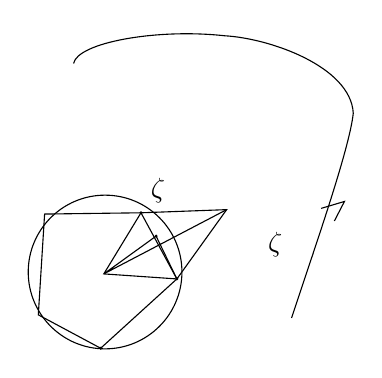
\begin{tikzpicture}[scale=.8,thin]
\coordinate (O) at (0,0);
\draw (.02,.03) circle (1.22);
\draw (-.94,.95)--(.59,.97)--(1.16,-.08)--(-.05,-1.18)--(-1.04,-.65)--cycle;
\draw (O)--(.59,.97) node[above right] {$\zeta$}--(1.95,1.02)--(1.16,-.08)--cycle;
\draw (O)--(1.95,1.02) (O)--(.83,.60)--(1.16,-.08);
\foreach \x/\y in {.59/.97,.83/.60,1.16/-.08,-.05/-1.18}{\fill (\x,\y) circle (.026);}
\node at (2.72,.47) {$\zeta$};
\draw (2.98,-.70) .. controls (3.33,.36) and (3.90,1.98) .. (3.96,2.55)
 .. controls (3.92,3.29) and (2.64,3.74) .. (1.92,3.78)
 .. controls (.83,3.90) and (-.42,3.67) .. (-.48,3.34);
\draw (3.45,1.04)--(3.82,1.15)--(3.66,.84);
\end{tikzpicture}}

\[
\begin{aligned}
{\unsure{\xi|\zeta}}^2-\frac1{\sin^2\frac{\pi}{5}}\xi
 +\frac18\frac{1-(-1)}{\sin^4\frac{\pi}{5}}&=0\\
\text{\unsure{i.e}} \qquad
 \xi^2-\frac1{\tfrac14(\unsure{2-\alpha|2+\alpha})}\xi
 +\frac14\frac1{5/16(1-\alpha)}&=0
\end{aligned}
\]

\[
 \zeta=\alpha/2+i\underbrace{\sqrt{1-\frac{\alpha^2}{4}}}_{1/2\sqrt{4-\alpha^2}}
 =\alpha/2+i/2\sqrt{\alpha+3}
\]

\[
 \deleted{\alpha^2+\alpha-1=0}\qquad \uline{NB}\qquad 4-\alpha^2=3+\alpha
\]

\[
 \xi^2-\frac{4(2-\alpha')}{(2-\alpha)(2-\alpha')}\xi
 +\frac45\frac{(1-\alpha')}{(1-\alpha)(1-\alpha')}
\]

\[
\begin{aligned}
 |\zeta+1|^2&=(1+\alpha/2)^2+\left(\frac{\sqrt{\alpha+3}}2\right)^2\\
 &=1+\alpha+\underbrace{\frac{\alpha^2}4+\frac{\alpha+3}4}_{\unsure{1/2|1}}\\
 &=\frac32+\alpha+
\end{aligned}
\]

\[
\begin{aligned}
N(2-\alpha)&=4-1+2=5\\
N(1-\alpha)&=1-1+1=1\\
-\alpha'&=+1+\alpha\\
2-\alpha'&=3+\alpha\\
1-\alpha'&=2+\alpha
\end{aligned}
\]

\[
 \sin\frac{\pi}{5}=\frac{1+\alpha/2}{\sqrt{3/2+\alpha}}
 =\deleted{\unsure{\tfrac12|\tfrac14}}\frac{(\alpha+2)}{3+2\alpha}\sqrt{3/2+\alpha}
 =\alpha\sqrt{3/2+\alpha}=\deleted{\unsure{\sqrt{(3/2)\alpha^2+\alpha^2}}}
\]

\[
 \underbrace{N(3+2\alpha)}_{\shortparallel\ (3+2\alpha)(3+2\alpha')}=9\unsure{-|+}\deleted{\unsure{4}}4-6=-1
\]

\[
\begin{aligned}
 \sin^2\left(\frac{\pi}{5}\right)&=\alpha^2(3/2+\alpha)=(1-\alpha)(3/2+\alpha)\\
 &=3/2-1/2\,\alpha\underbrace{-\alpha^2}_{\alpha-1}=\tfrac12(\alpha+1)
\end{aligned}
\]

\[
\begin{aligned}
 \frac{\alpha+2}{3+2\alpha}&=-(\alpha+2)(3+2\alpha')=-(\alpha+2)(1-2\alpha)\\
 &=-[\underbrace{-2\alpha^2}_{2\alpha-2}-3\alpha+2]=\alpha
\end{aligned}
\]

\[
 \deleted{\unsure{\xi^2-}}
\]

\[
\begin{aligned}
 \xi^2-\left[\tfrac45(3+\alpha)\right]\xi+\left(\tfrac45(2+\alpha)\right)&=0\\
 \xi=\tfrac{\deleted{\unsure{4}}2}{5}(3+\alpha)
 \mathbin{\pm}\tfrac25\sqrt{\deleted{\unsure{\tfrac4{25}}}(3+\alpha)^2-
 \deleted{\unsure{\tfrac15}}5(2+\alpha)}
 &=\tfrac25(3+\alpha)\mathbin{\pm}\sqrt{-5\alpha}
\end{aligned}
\]

\[
 \deleted{\unsure{28}}\qquad
 \deleted{9}+6\alpha+\underbrace{\alpha^2}_{\deleted{1}-\alpha}-\deleted{10}
 -\unsure{15|5}\alpha=\deleted{\unsure{-5\alpha|5\alpha}}
\]
% archive sheet number: 71
\scanpage{73}
\[
 \boxed{(5,3,5)}\quad\text{et}\quad\boxed{3,5,5}
\]

\[
\begin{aligned}
\theta_0&=\frac{2\pi}{5}\\
\theta_1&=\frac{2\pi}{3}\\
\theta_1-\theta_0&=\frac{4\pi}{15}\ ;\quad \frac{\theta_1-\theta_0}{2}=\frac{2\pi}{15}\\
\cos\Bigl(\frac{\theta_1-\theta_0}{2}\Bigr)&=\cos\theta\unsure{.|,}
\end{aligned}
\]

\[
\begin{aligned}
 \underbrace{\cos\frac{\deleted{\unsure{2}}2\pi}{15}}_{\frac{\alpha}4+\frac14\sqrt{9+3\alpha}}
 +\underbrace{\overbrace{\cos\frac{\pi}{5}}^{1/2(1+\alpha)}}_{\deleted{\unsure{\frac12\sqrt{2+\alpha}|\sqrt{2+\alpha}}}}
 &\overset{?}{\geq}2\sin\frac{\pi}{5}\overbrace{\sin\frac{\pi}{3}}^{\sqrt3/2}\\
 \deleted{\unsure{1+\alpha|1+2\alpha}}\qquad
 \frac12+\frac{3\alpha}4+\frac14\sqrt{9+3\alpha}
 &\qquad\frac{\sqrt3}{2}\sqrt{3+\alpha}\ \deleted{\sqrt3}
 =\frac12\underbrace{\sqrt{9+3\alpha}}_{\deleted{\unsure{\alpha+6}}}
\end{aligned}
\]
\unsure{NB}\,$\nearrow$

\[
\begin{aligned}
2\cos^2\frac{\pi}{5}&=1+\cos\frac{2\pi}{5}=1+\alpha/2=\tfrac12(2+\alpha)
 \ \unsure{\Rightarrow|,\!}\ 4\cos^2\frac{\pi}{5}=2+\alpha=(1+\alpha)^2,\quad
 \cos\frac{\pi}{5}=\tfrac12(1+\alpha)\\
\cos\frac{\pi}{5}&=\tfrac12\alpha\qquad
 \sin^2\frac{\pi}{5}=1-\tfrac14\alpha^2=\tfrac14(4-\alpha^2)=\tfrac14(3+\alpha)
\end{aligned}
\]

\[
\begin{aligned}
 &\deleted{\sin\frac{\pi}{5}=\sqrt{1-\frac{\alpha^2}{4}}}\\
 &\alpha^2+\alpha-1=0\\
 &\alpha=\tfrac12(\sqrt5-1)\leq\tfrac23\\
 &\deleted{\text{car }\sqrt5\leq3}\\
 &\text{car }\sqrt5\leq\tfrac43+1=\tfrac73\\
 &\text{i.e.}\quad5\leq\tfrac{49}{9}\quad\text{i.e.}\quad45\leq49\ !
\end{aligned}
\]

\[
\begin{aligned}
 \tfrac14\sqrt{9+3\alpha}&\overset?{\leq}\tfrac12+\tfrac{3\alpha}4
 +\deleted{\unsure{\tfrac12\sqrt{2+\alpha}}}\\
 \sqrt{9+3\alpha}&\leq 3\alpha+2\quad
 \deleted{\unsure{\sqrt{2+\alpha}(1+\alpha)}}\quad \deleted{\unsure{=(\alpha+1)^2}}\\
 9+3\alpha&\leq\overbrace{9\alpha^2}^{9-9\alpha}+4(\deleted{\unsure{4}}1+\unsure{6\alpha|3\alpha})
 =\deleted{\unsure{5+3\alpha}}\\
 &\deleted{\unsure{1+4\alpha\sqrt{2+\alpha}}}\quad \deleted{13-5\alpha}\\
 \deleted{9+8\alpha\leq{}}&\deleted{\unsure{\shortparallel}}\quad\deleted{-\alpha+8+4\alpha}\\
 &\deleted{+4\sqrt{\underbrace{2\alpha+\alpha^2}_{1+\alpha}}}\\
 &\deleted{=9+3\alpha+4\sqrt{1+\alpha}}\\
 &=13-3\alpha\\
 \deleted{\text{OK}}\quad&6\alpha\leq4\qquad\alpha\leq\tfrac23\quad\text{OK}
\end{aligned}
\]

\[
\begin{aligned}
 \frac{\theta_1-\theta_0}{2}&=\frac{\pi}{5}-\frac{\pi}{3}\\
 \cos\bigl(\uparrow\bigr)&=\underbrace{\cos\frac{\pi}{5}}_{\alpha/2}
 \underbrace{\cos\frac{\pi}{3}}_{1/2}
 +\underbrace{\sin\frac{\pi}{5}}_{\frac12\sqrt{3+\alpha}}
 \underbrace{\sin\frac{\pi}{3}}_{\sqrt3/2}\\
 &=\frac{\alpha}{4}+\frac14\sqrt{9+3\alpha}
\end{aligned}
\]

\deleted{Reste $(3,5,5')$}

\[
 \boxed{(5,3,5')}\quad\text{et}\quad\boxed{(3,5,5')}
\]

% slanted
\margin{\deleted{\uuline{à élucider} (\unsure{Cas effectifs} \unsure{pythagoricien|pythagoriciens} ?)}}

même calcul, sauf que \deleted{\unsure{dans|ici}}
$\cos\frac{\theta}{2}=\cos\frac{\pi}{5}=\tfrac12\deleted{\unsure{\sqrt{\vphantom1}}}(1+\alpha)=-\tfrac12\alpha'$
dans le \unsure{mb|mbr} de gauche, doit être remplacé par
$\cos\frac{2\pi}{5}=\frac12\deleted{\unsure{\tfrac12}}\alpha\deleted{\unsure{avec}}$
\deleted{$=\tfrac12\sqrt{1-\alpha}$} \deleted{$=\alpha/2$}
qui est plus petit, il faut vérifier

\[
\begin{aligned}
 \deleted{\tfrac14}\sqrt{9\unsure{-|+}3\alpha}
 &\leq\deleted{\unsure{\tfrac12\alpha\sqrt{1-\alpha}+\tfrac{\alpha}4}}-\tfrac{\alpha}{4}
 \quad\text{pas vrai !}\\
 9+3\alpha&\leq4(1-\alpha)+\alpha^2+4\sqrt{\alpha^2(1-\alpha)}
\end{aligned}
\]
% archive sheet number: 72
\scanpage{74}
\[
 \text{Cas}\quad\boxed{5,5,5}\qquad
 1+\underbrace{\cos\frac{\pi}{5}}_{1/2(1+\alpha)}
 \geq\underbrace{2\sin^2\frac{\pi}{5}}_{1/2(3+\alpha)}
\]

\deleted{i.e. \quad $3+\alpha$}\qquad On a égalité

OK.

Seul cas indéterminé est celui de \uline{$(5,3,5')$} et \uline{$(3,5,5')$} -- vérifier s'il existe bien -- si oui, il faut trouver comment éliminer \unsure{le|les} \unsure{$\}$|$\xi$|$\int$} indésirable \ldots.
% archive sheet number: 73
\scanpage{75}
(6 p)

2-Polyèdres réguliers finis en car. $0$ (classification)
% archive sheet number: 74
\scanpage{76}
Nous nous intéressons au cas $n=2$, et au cas où $G_0$ est fini et \deleted{\unsure{admet une représentation}}\inserted{a sa représentation en $\operatorname{Aut}(X)$} \uline{fidèle} \deleted{\unsure{comme dans} $\operatorname{Aut}(X)$} (peut-être pas dans $\operatorname{Aut}(C)$. -- il peut y avoir un noyau non trivial pour $G_0\unsure{\text{---}|\longrightarrow}\operatorname{Aut}(C)$]

\[
 \left\{\begin{aligned}
 &\text{Invariants}\qquad\beta_0=\alpha_0+2,\quad\beta_1=\alpha_1+2\\
 &\rho=8-2(\beta_0+\beta_1)=-2(\alpha_0+\alpha_1)\qquad\widetilde\rho=-(\alpha_0+\alpha_1)\\
 &\sigma=4-\beta_1=2-\alpha_1,\quad\sigma'=4-\beta_0=2-\alpha_0
 \end{aligned}\right.
\]

$Q_C=Y$ de dim relative $1$, lisse sss $\beta_0\beta_1\widetilde\rho$ inv, i.e. sss en tout point on a \deleted{\unsure{$\alpha_0$}}\inserted{$\alpha_0\ne-2,\alpha_1\ne-2,$} $\alpha_0+\alpha_1\ne0$

$Q_X$ de dim relative $2$, lisse sss $\beta_1\beta_1\sigma$ inv, i.e. sss en tout point on a

\[
 \alpha_0\ne-2,\quad\alpha_1\ne\pm2,
\]

\[
\begin{aligned}
 \rho_f&=\tau_0\tau_1\quad\text{son ordre dépend de la façon connue de }\beta_0=\alpha_0+2\\
 \rho_s&=\tau_1\tau_2\hspace{46mm}\beta_1=\alpha_1+2,
\end{aligned}
\]

\deleted{\unsure{D'autre|D'où}} \unsure{On} sait que

% slanted
\margin{vérifier si \unsure{$Q$|$\varnothing$} non lisse}

\[
 \underline{\operatorname{Aut}}(C,Q_C)\overset{\sim}{\longrightarrow}
 \underline{\operatorname{Aut}}(Q_C)=\operatorname{Aut}(Y)
\]

Donc la cat. des 2-polyèdres réguliers \deleted{\unsure{et sur $S$}}\inserted{\unsure{paramétrés}} épinglés sur $S$ \inserted{rel. à $G_0$} est équivalente à celle des triples $(Y,\varphi_{G_0}^{Y})$ d'une \unsure{cônique|conique} $Y$ sur $S$ et d'un hom.

% slanted
\margin{$G_0$ fini ou non, mais il faut supposer $(\beta_0,2)\mathcal O_S=\mathcal O_S$ i.e. $\beta_0\ne0$ aux pts de car. $2$}

\[
 \varphi_{G_0}^{Y}:G_0\longrightarrow\operatorname{Aut}(Y),
\]

satisfaisant les conditions

a) \deleted{\unsure{$\tau_0,\tau_1,\tau_2$}} $\rho_s^2\ne1,\ \rho_f^2\ne1$ en \unsure{toute|toutes} fibre ($\Rightarrow\tau_0,\tau_1,\tau_2\ne\mathrm{id}$ sur \unsure{tte} fibre, donc $\tau_0,\tau_1,\tau_2$ des \uline{réflexions})

% slanted
\margin{$2$ \deleted{\unsure{pour que}} a) (avec b) \deleted{soit} \uline{suffisant} pour que \deleted{ça provienne d'une} structure de polyèdre régulier, il faut se limiter au cas où $\deleted{\unsure{\rho=}}\beta_0\beta_1$ inv (les $\tau_i^C$ sont des réflexions \deleted{\unsure{affines}} \deleted{\unsure{droites}} orthogonales)}

b) Les sections $h_0,h_1,h_2$ de $C$ définies par $\tau_0,\tau_1,\tau_2$ sont non alignées en tout point. \deleted{Si}

Si $\beta_0$ inv et $(\beta_1,4-\beta_0)\mathcal O_S=\mathcal O_S$ [i.e. \deleted{\unsure{$\beta_1$, en un pt, on a}} \inserted{en aucun pt on n'a} à la fois \deleted{\unsure{$\beta_1=0,\beta$}} $\alpha_1=-2,\alpha_0=2$], alors b) équivaut à

b') En tout pt, la repr. $\varphi_{G_0}^C$ \deleted{\unsure{est}} a pas de droite fixe.

Si $Y$ lisse, i.e. \deleted{\unsure{$\beta_0,\beta_1,\widetilde\rho$, de}}\inserted{en aucun} pt on n'a \deleted{\unsure{simultanément}}\inserted{l'une des égalités} $\alpha_0=-2,\alpha_1=-2,\alpha_0+\alpha_1=0$, alors la condition b') équivaut à :

b'') \inserted{Sur aucune fibre} Il n'existe \deleted{pas} de $2$-diviseur stable pour $\varphi_{G_0}^{Y}$.
% archive sheet number: 75
\scanpage{77}
I) \unsure{Condition|Conditions} de finitude, sur corps de base $k$

\uline{Prop.} Si $G_0$ est fini, alors \deleted{\unsure{les}} $\beta_0,\beta_1$ sont algébriques sur le corps premier. L'inverse est vrai si \deleted{$p=$} $\operatorname{car}.k>0$.

% slanted
\margin{valable en dim quelconque}

\deleted{\uline{\unsure{Raisons|Racines}} \unsure{de ce que}}

Introduisons \deleted{\unsure{les val propres}}\inserted{des solutions} (dans une clôture alg. $\bar k$ de $k$) $\zeta_i$ $(i=0,1)$ de l'équation aux val. propres

\[
 \zeta_i^2-\alpha_i\zeta_i+1=0\qquad\text{i.e.}\quad \zeta_i+\zeta_i^{-1}=\alpha_i
\]

Donc pour $i=0,1$ fixé, $\zeta_i$ est déterminé mod passage à $\zeta_i^{-1}$.

\[
 \text{Soit}\qquad\unsure{\nu'_i|\nu_i}=\text{ordre de }\zeta_i\qquad i=0,1
\]

Donc $\nu_i$ est tjrs premier à $p$, sauf si $\nu'_i=1$ i.e. $\zeta_i=1$, i.e. $\alpha_i=2$.

\unsure{Rappelons}

\uline{Prop} a) Si $\nu'_i\ne\deleted{\unsure{1}}\inserted{1,2}$ \deleted{\unsure{alors}} \inserted{i.e. $\alpha_i\ne\pm2$ i.e. $\beta_i(4-\beta_i)\ne0$,} alors $\nu_i=$ ordre de $\rho_i$

(\uline{NB} $\rho_0=\rho_f,\rho_1=\rho_s$)

b) Si \deleted{\unsure{$\nu'_i=2$}}\inserted{i.e. $\alpha_i=-2$, i.e. $\deleted{\unsure{\alpha}}\beta_i=0$ ($\nu'_i=2$, ou $\nu'_i=1$ en car $2$)} alors $\rho_i$ d'ordre $2p$

c) \deleted{Si \unsure{$\nu'_i=1$} en car \unsure{$p$} $\alpha_i=2\ne-2$, \unsure{$\rho_i$} alors $\left\{\begin{smallmatrix}\nu_i=p&\text{si }p\ne2\\\nu_i=\unsure{1}&\text{si }p=2\end{smallmatrix}\right.$}
Si $\alpha_i=2\ne-2$ (i.e. $\nu'_i=1$ en car. $\ne2$) alors $\nu_i=p$

[\,\uline{NB} Dans b) et c), on convient que $p=+\infty$ dans cas de car. nulle\,]

\uline{Théorème} Supposons $k$ de car. $0$. Pour que $G_0$ soit fini, il f et s. que l'on soit dans l'un des \deleted{quatre}\inserted{six} cas suivants

\deleted{1) $\nu_0=3,\nu_1=3$ (tétraèdre)}
\deleted{2) $\nu_0=3,\nu_1=4$ (octaèdre) \quad 2') $\nu_0=4,\nu_1=3$ (cube)}
\deleted{3) $\nu_0=3,\nu_1=5$ (icosaèdre) \quad 3') $\nu_0=5,\nu_1=3$ (dodécaèdre)}
\deleted{\unsure{2) $\nu_0=3,\nu_1=$}}

% slanted
\margin{on appellera ces cas les cas pythagoriciens (\unsure{sur base quelconque|cas base quelconque})}

\[
 \mathrm{I})\quad\nu_0=3,\ \nu_1=3\quad(\text{tétraèdre})\qquad
 \text{i.e. }\alpha_0=\alpha_1=-1,\quad\text{i.e. }\beta_0=\beta_1=+1\ \searrow
\]

\[
 \mathrm{II})\quad\nu_0=3,\ \nu_1=4\quad(\text{octaèdre})\qquad
 \text{i.e. }\alpha_0=-1,\alpha_1=0\quad\text{i.e. }\beta_0=1,\beta_1=2
\]

\[
 \mathrm{III})\quad\nu_0=3,\ \nu_1=5\quad(\text{icosaèdre})\quad
 \text{i.e. }\alpha_0=-1,\ \alpha_1\deleted{\unsure{=\alpha}}\text{ solution de l'équation }
 \boxed{\alpha_1^2+\alpha_1-1=0}
\]

\[
 \mathrm{II}')\quad\nu_0=4,\ \nu_1=3\quad(\text{cube})\qquad
 \text{i.e. }\alpha_0=0,\alpha_1=-1\quad\text{i.e. }\beta_0=2,\beta_1=1
\]

\[
 \mathrm{III}')\quad\nu_0=5,\ \nu_1=3\quad(\text{dodécaèdre})\quad
 \text{i.e. }\alpha_0\text{ solution de }\boxed{\alpha_0^2+\alpha_0-1=0},\quad
 \alpha_1=-1\ \text{i.e. }\beta_1=1
\]

\[
 \mathrm{IV})\quad\nu_0=\nu_1=5,\ \uline{\text{et}}\ \alpha_0\ne\alpha_1\
 \overset{\text{(pentagramme)}}{\vphantom{I}}\quad\text{i.e. }\alpha_0,\alpha_1
 \text{ solutions }\uline{\text{distinctes}}\text{ de }\boxed{\alpha^2+\alpha-1=0}
\]
% archive sheet number: 76
\scanpage{78}
\uline{Remarque} Les cas I, II \inserted{\deleted{\unsure{et}} II'} correspondent \inserted{chacun} à une structure, définie à isom. (unique près), \inserted{qui existe \deleted{pour} $\forall\,k$ de car $0$ (i.e. définie sur $\mathbb Q$)} les autres \inserted{trois} correspondent chacun à deux structures, définies à isom unique près, \deleted{celles} qui \unsure{existe|existent} ssi $k$ contient une solution de $\alpha^2+\alpha-1=0$, i.e. ssi $k$ contient le corps $\tfrac12$ cyclotomique d'indice $5$. Il y a donc en tout $3+3\times2=$\uuline{$9$} types d'isomorphie de ``polyèdres réguliers finis'' sur corps $k$ de car $0$, contenant $\alpha$.

\uline{\unsure{Indication|Indications} sur dém. du th.} \deleted{\unsure{Lisse :|Lisons}} OPS \inserted{$k$ alg. clos, et $=$} $k=\mathbb C$.

I) Notons d'abord que d'après la prop, si valeurs $\nu_0,\nu_1$ sont finies, on a \deleted{\unsure{$\beta_0\beta_1$ inv}} $\alpha_0\ne\pm2,\alpha_1\ne\pm2$

\deleted{\unsure{d'où} $\sigma,\sigma'\ne0$, donc $Q_X$ lisse. Peut-on avoir $\rho=0$ i.e. $\alpha_0+\alpha_1=0$ ? i.e. $\alpha_1=-2\alpha_0$ \quad $\alpha_0=\alpha,\alpha_1=-\alpha$, où $\alpha$ est une solution d'une équation $\tfrac12$ cyclotomique (donnée par un indice $\nu=\nu_0\geq\unsure{3|2|3/2}$ ? Comme \unsure{$\rho\ne0$} $\sigma=2-\alpha_1=2\alpha\ne0$, on serait dans un cas où $Q_E=Q\setminus Q\cap C=Q\setminus Y$ est un plan \unsure{euclidien}}

Les $\alpha_i$ sont solutions d'équations $\tfrac12$-cyclotomiques d'indices $\nu_0,\nu_1\geq3$. Ces solutions sont \uline{réelles}, donc la situation provient d'une situation sur $k_0=\mathbb R$. Comme on prend $G_0$ \deleted{\unsure{est|étant}} fini, $\exists$ forme quadratique invariante définie positive sur $V$, \deleted{\unsure{et sur $E$ donc}} $\boxed{\beta\rho\ne0}$ i.e. \uline{$Y$ lisse}.

$\unsure{\mathbb G_0|G_0|\underline G_0}\subset\operatorname{GP}(1,\mathbb C)$ groupe fini d'autom de $Y\simeq\mathbb P^1_{\mathbb C}$, \deleted{\unsure{utilisons}} soit $Z=Y/G_0$ \inserted{$\simeq\mathbb P^1_{\mathbb C}$} \unsure{Utilisant|Utilisons} \unsure{Hurwicz|Hurwitz} on trouve que $Y$ est ramifié sur $Z$ en $2$ ou trois points \inserted{exactement}. Dans le cas de $2$ pts, on aurait au dessus \unsure{des|de} ceux-ci un diviseur de degré $2$ stable sous $G_0$, absurde. Donc il y a trois points de ramification, et la formule de Hurwicz nous dit que les \deleted{\unsure{indices de}} indices de ramification sont $(2,p,q)$ -- les couples $(p,q)$ sont \inserted{parmi} ceux inventoriés plus haut, \inserted{savoir} $(3,3)(3,4)(3,5)$ \deleted{(et} (à \unsure{la} symétrie près), plus $(2,\unsure{2|p},p)$ (cas diédral) -- mais dans celui-ci, il y a au dessus des

\margin{$\mathbb G_0=\operatorname{Im}G_0$, $G_0\to\mathbb G_0$ de noyau d'ordre 1 ou 2.}
% archive sheet number: 77
\scanpage{79}
pt de ramification d'indice $p$ un diviseur de degré $2$ stable par $G_0$, encore absurde. Donc on est dans l'un des trois cas, $(2,3,3),(2,3,4),(2,3,5)$.

II) \deleted{\unsure{Considérons} \unsure{Au} \unsure{voisin}}\inserted{Nous allons} montrer que ces trois cas \inserted{de ss-groupes finis de $\operatorname{GP}(1,\mathbb C)$} correspondent à des classes de conjugaison bien déterminées de ss-groupes de $\operatorname{GP}(1,k)$ : groupes tétraédral, octahédral, icosaédral.

Pour ceci, considérons les couples $(\nu_0,\nu_1)$ correspondants (cas I, II, III) \deleted{\unsure{en|---}} choisissant dans le cas III $\alpha=\zeta+\zeta^{-1}$, où $\zeta=\exp\frac{2i\pi}{5}$, donc $\alpha=2\cos\frac{2\pi}{5}$. Les \deleted{\unsure{vérifions que les}}\inserted{\unsure{supposons connus|supposés connus}} les polyèdres réguliers \unsure{combinatoires|correspondants} \unsure{s'identifiant|s'identifient} aux tétraèdre, octaèdre, icosaèdre -- on constate aisément, sur les formules explicites qu'on trouve des réalisations géom \inserted{strictement} fidèles de ceux-ci. Leurs groupes \inserted{$G_0$} sont respectivement

$\unsure{\mathfrak S_4|\mathscr S_4},\ \mathfrak S_4\times\mathbb Z/2\mathbb Z,\ \mathfrak A_5\times\mathbb Z/2\mathbb Z$, et \deleted{\unsure{l'}}\inserted{les} images de celui-ci dans $\operatorname{GP}(1,k)$ \deleted{est} sont respectivement $\simeq\unsure{\mathfrak A_4|\mathfrak S_4},\mathfrak S_4,\mathfrak A_5$

Appelons ceux-ci les groupes pythagoriciens standart dans $\operatorname{GP}(1,k)$ (définis mod conjugaison). Ceci a établi \inserted{en passant} l'existence des cas I, II, III, et par dualité II') III') -- \deleted{l'unicité}

Il reste à prouver que le seul cas de pol. régulier fini qui n'est pas couvert par les précédents est le cas IV -- et d'en prouver l'existence de IV. Or \inserted{pour \unsure{celle-ci|celui-ci},} la construction du pentagramme associé à un icosaèdre est bien claire. -- cf plus bas la forme que prend cette construction dans notre contexte actuel

\deleted{III) Revenons au cas de $G_0\subset\operatorname{GP}$ \unsure{, engendré par|, engendré pour} $\tau_0,\tau_1,\tau_2$, fini.}
% archive sheet number: 78
\scanpage{80}
\deleted{III) Notons maintenant que dans les trois cas I II III envisagés, faisant la construction sur $\mathbb R$ et $\mathbb C$, on trouve des cartes cellulaires régulières sur la sphère -- qui est \uline{simplement connexe}. On en déduit \inserted{par la théorie des cartes} que le groupe $G_0^+$ \inserted{$(=\mathfrak A_4,\mathfrak S_4,\mathfrak A_5)$} est engendré par les gén. $\rho_s,\rho_f$ avec les seules relations $\rho_f^{\nu_0}=\rho_s^{\nu_1}=(\rho_f\rho_s)^2=1$. La théorie}

% slanted
\margin{$\bigcirc$ on pourrait sans doute l'obtenir \unsure{directement}}

\deleted{\unsure{au cas} \illegible{5} II, III,} du groupe fondamental de la sphère moins trois pts, \deleted{\unsure{IV A la} \illegible{2} I, \unsure{ou}}

\deleted{III} montre alors que dans le cas général, le ss-groupe fini $G_0$ \deleted{\unsure{engendré}} doit être un \uline{quotient} d'un des gpes $\mathfrak A_4,\mathfrak S_4,\mathfrak A_5$ -- ceci implique déjà que les ordres de ses éléments sont $\leq5$, donc

\[
 \boxed{3\leq\nu_0,\nu_1\leq5}
\]

D'ailleurs, exprimant (sur $k_0=\mathbb R$) que la forme quadratique de matrice (matrice par r. à $a_0,a_1,a_2$)

\[
 \begin{pmatrix}
 2 & -\deleted{\unsure{2}}\beta_0 & 0\\
 -\deleted{\unsure{2}}\beta_0 & 2\beta_0 & -\deleted{\unsure{2}}\beta_0\beta_1\\
 0 & -\deleted{\unsure{2}}\beta_0\beta_1 & 2\beta_0\beta_1
 \end{pmatrix}
\]

est définie positive, on trouve les conditions

\[
 \deleted{\unsure{\beta_0>0,\beta_1>0|\beta_0,\beta_1>0}}\qquad
 4-(\beta_0+\beta_1)>0\qquad\beta_0(4-\beta_0)>0
\]

\[
 \text{i.e}\qquad\left\{\begin{aligned}
 &\alpha_0+\alpha_1<0\\
 &\deleted{\unsure{\alpha_0^2<4}}\ \text{\unsure{i.e.}}\quad -2<\alpha_0,\alpha_1\unsure{<|\leq}+2
 \end{aligned}\right.
\]

(Conditions néc. et suff pour que la forme \unsure{envisagée|env. géom} soit définie, pour des \deleted{\unsure{couples}} $\alpha_0,\alpha_1$ réels).
% archive sheet number: 79
\scanpage{81}
En fait, les relations $-2<\alpha_0,\alpha_1<+2$ sont satisfaites automatiquement, si $\alpha_0,\alpha_1$ solutions d'équations $\tfrac12$ cyclotomiques, correspondant à $\nu_0,\nu_1\ne1,2$ i.e. $\nu_0,\nu_1>3$. Quitte à passer au système dual, on est donc amené à regarder les possibilités, où

\[
 3\leq\nu_0\leq\nu_1\leq5
\]

A priori, il y a \deleted{\unsure{$(3,4)(3,5$|$(3,3)(3,5)$}} $(3,3)(3,4)(3,5)$ (cas I II III) $(4,4),(4,5)$ et $(5,5)$. Or $(4,4)$ correspond à \deleted{\unsure{$(0,0$}} $\alpha_0=\alpha_1=0$, $\alpha_0+\alpha_1=0$, impossible, et $(4,5)$ à $\alpha_0=0,\alpha_1=\tfrac12(-1\pm\sqrt5)$. Mais \uline{OPS} $\alpha_1=\tfrac12(-1\underline{\underline{+}}\sqrt5)$ qui est $>0$, \deleted{on a gagné} impossible ! Enfin considérons le cas $5,5$ OPS $\alpha_0=\tfrac12(-1\underline{\underline{+}}\sqrt{\unsure{5|6}})>0$, donc il faut $\alpha_1<0$ donc $\alpha_{1}=\tfrac12(-1-\sqrt{\deleted{\unsure{5}}5})$ ($\alpha_0+\alpha_1=-1$ OK).

On a gagné !
% archive sheet number: 80
\scanpage{82}
(12 p)

Opérations sur systèmes de Schwartz
% archive sheet number: 81
\scanpage{83}
Soit $\Pi_0$ le groupe engendré par les générateurs $\underline{\unsure{h|\ell}}_0,\underline h_1,\underline h_2$, soumis à

\[
 \underline h_0\,\underline h_1\,\underline h_2=1
\]

et soit $\deleted{\unsure{\widehat{\vphantom\Pi}}}\widehat\Pi$ son complété profini. Un hom de $\Pi_0$ dans un groupe $H$ (ou de $\widehat\Pi$ ds un gpe $H$ fini) équivaut à la donnée de

\[
 h_0,h_1,h_2\in H\qquad\text{satisfaisant}\quad h_0h_1h_2=1
\]

\margin{Soit $\mathcal T(H)\inserted{\subset H^3}$ l'ens des ces triples}

L'hom $\Pi_0\text{---}H$ ($\widehat\Pi\unsure{\text{---}|\longrightarrow}H$) est surjectif ssi $(h_0,h_1,h_2)$ est un syst. de \unsure{Schwartz|Schwarz}

\margin{$\operatorname{Sch}(H)\subset\mathcal T(H)$}

Soit \deleted{$\Pi$ le groupe des}

\diagram{\begin{tikzcd}[ampersand replacement=\&,column sep=tiny,row sep=small]
 \Omega_0 \arrow[d] \& {}=\operatorname{Aut}(\Pi_0)\\
 \Omega \& {}=\operatorname{Aut}(\widehat\Pi)
\end{tikzcd}}

Alors $\Omega_0$ (resp. $\Omega$, si $H$ fini) opère \inserted{à droite} sur \inserted{$\mathcal T(H)\simeq$} $\underline{\operatorname{Hom}}(\Omega,H)$ (\deleted{\unsure{sur}} $\simeq\underline{\operatorname{Hom}}(\widehat\Omega,H)$ \inserted{si $H$ fini}) et sur le sous-ensemble $\operatorname{Schw}(H)$. On a

\diagram{\begin{tikzcd}[ampersand replacement=\&,row sep=small,column sep=small]
 \& \& \& \operatorname{Autext}(\Pi_0)\arrow[d,equal] \&\\
 1\arrow[r,dash] \& \deleted{\unsure{\Pi}}\unsure{\Omega|\Pi}_0\arrow[r,dash] \& \Omega_0\arrow[r] \& \widetilde\Omega_0\arrow[r] \& 1\\
 1\arrow[r,"?",dash] \& \widehat\Pi\arrow[r,dash] \& \Omega\arrow[r] \& \widetilde\Omega\arrow[r,dash]\arrow[d,equal] \& 1\\
 \& \& \& \operatorname{Autext}(\widehat\Omega) \&
\end{tikzcd}}

et deux éléments de \deleted{$\underline{\operatorname{Hom}}(\Omega,H)$}\inserted{$\mathcal T(H)$} conjugués sous $\Pi$ ($\widehat\Pi$) sont conjugués dans $H$ -- l'inverse étant vrai pour les éléments de $\operatorname{Schw}(H)$. Ainsi $\widetilde\Omega_0$ ($\widetilde\Omega$) opère sur $\widetilde{\mathcal T}(H)=\mathcal T(H)/H$ et sur $\widetilde{\operatorname{Sch}}(H)=\operatorname{Sch}(H)/H=\operatorname{Sch}(H)/\underset{\text{ou }\widehat\Pi}{\Pi_0}$.

\deleted{\unsure{Dans le cas}} Dans une énumération des syst. de Schwartz relatifs à $H$, il convient de tenir compte des opérations (\unsure{ou} au \uline{moins} \unsure{quelques unes|quelques-unes}) de $\Omega_0$, ou $\Omega$ -- et de de $=$ pour $\widetilde\Omega_0,\widetilde\Omega$ quand on envisage $\widetilde{\operatorname{Sch}}(H)$.

\deleted{\unsure{$0\longrightarrow S_3\longrightarrow{}$} \unsure{$1\to\Omega\to S_3$}}
% archive sheet number: 82
\scanpage{84}
$\mathfrak S_3$ opère (\unsure{fid\textsuperscript{t}|fidt}) sur $\deleted{\unsure{\Pi}}\Omega_0$ \unsure{plutôt|puis} $\Pi$ par

\[
 \sigma(h_i)=\begin{cases}
 h_{\sigma(i)}&\text{si }\sigma\in\mathfrak S_3^+\\
 h_{\sigma(i)}^{-1}&\text{si }\sigma\in\mathfrak S_3^-
 \end{cases}
\]

On a donc des injections

\diagram{\begin{tikzcd}[ampersand replacement=\&,row sep=small]
 \mathfrak S_3\arrow[r,hook]\arrow[dr,hook]\&\Omega_0\arrow[d]\\
 \&\Omega
\end{tikzcd}}

d'où

\diagram{\begin{tikzcd}[ampersand replacement=\&,row sep=small]
 \mathfrak S_3\arrow[r,hook]\arrow[dr,hook]\&\widetilde\Omega_0\arrow[d]\\
 \&\widetilde\Omega
\end{tikzcd}}

[l'injectivité $\mathfrak S_3\unsure{-|\longrightarrow}\widetilde\Gamma$ est vérifiée immédiatement]

\[
 \text{Soit}\qquad\gamma_0=\mathbb Z^*,\qquad
 \gamma=\widehat{\mathbb Z}^{*}
\]

On va définir trois op. de $\gamma_0\times\gamma_0$ \deleted{sur} \unsure{ds} $\Omega_0$, et de $\gamma\times\gamma$ sur $\Omega$, \deleted{notées $\rho$} Si $\varepsilon,\varepsilon'\in\gamma_0\times\gamma_0$ ou $\gamma\times\gamma$, on notera par $\rho_{\bullet\varepsilon,\varepsilon'},\ \rho_{\varepsilon\bullet\varepsilon'},\ \rho_{\varepsilon,\varepsilon'\bullet}$ les effets de $(\varepsilon,\varepsilon')$ \deleted{\unsure{p}} par ces trois opérations. On pose

\[
\left\{\begin{aligned}
 \rho_{\varepsilon,\varepsilon'\bullet}(h_0)&=h_0^\varepsilon,&
 \rho_{\varepsilon,\varepsilon'\bullet}(h_1)&=h_1^{\varepsilon'}&
 \inserted{\text{donc}}\quad\rho_{\varepsilon,\varepsilon'}(\deleted{\unsure{t}}h_2)&=h_1^{-\varepsilon'}h_0^{-\varepsilon}\\
 \rho_{\deleted{\unsure{\varepsilon}}\bullet\varepsilon\varepsilon'}(h_1)&=h_1^\varepsilon,&
 \rho_{\bullet\varepsilon\varepsilon'}(h_2)&=h_2^{\varepsilon'}&
 \rho_{\bullet\varepsilon\varepsilon'}(h_0)&=h_2^{-\varepsilon'}h_2^{-\varepsilon}\\
 \rho_{\varepsilon'\bullet\varepsilon}(h_2)&=h_2^\varepsilon,&
 \rho_{\varepsilon'\bullet\varepsilon}(h_0)&=h_0^{\varepsilon'}&
 \rho_{\varepsilon'\bullet\varepsilon}(h_1)&=h_0^{-\varepsilon'}h_2^{-\varepsilon}
\end{aligned}\right.
\]

\deleted{On définit ainsi, si $I$ est une partie à deux él. de $\{0,1,2\}$} De façon plus intrinsèque, si $I$ est une partie à $2$ él. \deleted{\unsure{de}} de $\{0,1,2\}=\Delta_2$, on définit des hom

\diagram{\begin{tikzcd}[ampersand replacement=\&,row sep=tiny,column sep=small]
 \rho_0^I:\&\gamma_0^I\arrow[r]\arrow[d,hook]\&\unsure{\Gamma_0|\Pi_0}\arrow[d,hook]\\
 \rho^I:\&\gamma^I\arrow[r]\&\Gamma
\end{tikzcd}}

en \deleted{\unsure{posant, si}}\inserted{faisant opérer} $\varepsilon=(\varepsilon_i)_{i\in I}$ sur $\Omega_0$ (resp $\Omega$) par \deleted{l'action de $\varepsilon$}

\[
 \rho^I_{\unsure{\bullet|0}}(\varepsilon)(\underline h_i)=\underline h_i^{\varepsilon_i}\qquad(i\in I)
\]

\deleted{et prolonge} ce qui donne un autom de $\Omega_0\simeq\mathbb Z^{(*I)}$ -- puissance libre

Les relations entre les op. de $\mathfrak S_3$ et les $\rho^I$
% archive sheet number: 83
\scanpage{85}
\deleted{\unsure{sont les suivantes}}\inserted{s'expriment} comme suit : Si $\sigma\in\mathfrak S_3$, et $\widetilde\sigma_\Omega$ est l'op. sur $\Omega_0$ (ou $\Omega$), on a

\[
 \left\{\begin{aligned}
 \widetilde\sigma_\Omega\,\rho^I(\varepsilon)\,\sigma_\Omega^{-1}
 &=\rho^{\sigma I}(\sigma\varepsilon)\qquad\text{\unsure{i.e}}\\
 \sigma_\Omega\rho^I(\varepsilon)&=\rho^{\sigma I}(\sigma\varepsilon)\sigma_\Omega
 \end{aligned}\right.
\]

Ceci montre que le ss/groupe \inserted{de $\Gamma_0$ (ou $\widetilde\Gamma_0$, ou $\Gamma$, ou $\widetilde\Gamma$)} engendré par $\mathfrak S_3$ et un des $\rho^I(\gamma_0^I)$ (resp. $\rho^I(\gamma^I)$) / \deleted{\unsure{resp}} ou par $\mathfrak S_3$ et \deleted{\unsure{un}} les $3$ $\rho^I(\gamma_0^I)$ (resp $\rho^I(\gamma^I)$) \unsure{sont|est} le $=$, \deleted{\unsure{dits $\Gamma_0$|soit $\Gamma_0$}} $\Gamma_0^+,\widetilde\Gamma_0^+,\Gamma^+,\widetilde\Gamma^+$ ;

% slanted
\margin{/ il suffit $=$ de prendre $\mathfrak S_3$ et \uline{un} des $\rho^I(\gamma_0^{(i)})$ \deleted{$(i\in I)$} (sur les six possibilités)}

et \deleted{\unsure{si on désigne par}} \inserted{le groupe} engendré par les $\rho^I(\gamma_0^I)$ ($\rho^I(\gamma^I)$) en est un ss-groupe invariant \deleted{sont} les $\unsure{\mathbb E_0|\mathrm E_0|\mathbb E\mathrm l_0},\widetilde{\mathbb E}_0,\mathbb E,\widetilde{\mathbb E}$ \deleted{\unsure{$\Gamma_0^+$}} quotient des deux étant \deleted{\unsure{un}} (un groupe quotient de $\mathfrak S_{\unsure{4|3}}$ à priori, mais on voit aisément qu'il est égal à :] $\mathfrak S_3$, en fait c'est un produit $\tfrac12$ direct de $\mathfrak S_3$ et de celui-ci.

% slanted
\margin{(groupe des op. ``élémentaires'')}

\[
 \left\{\begin{aligned}
 \Gamma_0^+&\simeq\mathfrak S_3\underset{1/2}{\cdot}\mathbb E_0&
 \widetilde\Gamma_0^+&\simeq\mathfrak S_3\underset{1/2}{\cdot}\widetilde{\mathbb E}_0\\
 \Gamma^+&\simeq\mathfrak S_3\underset{1/2}{\cdot}\mathbb E&
 \widetilde\Gamma^+&\simeq\mathfrak S_3\underset{1/2}{\cdot}\widetilde{\mathbb E}
 \end{aligned}\right.
\]

\deleted{\uline{\unsure{Questions}}}

\uline{Construction} \unsure{Soient|Soit} $\mathfrak S,\gamma$ deux groupes. Considérons le produit libre $\mathcal L=\mathfrak S\deleted{\unsure{*}}*\gamma$. On a un hom

\[
 \mathcal L=\mathfrak S*\gamma\longrightarrow\mathfrak S
\]

dont le noyau est le ss-groupe \unsure{inv$=$|fermé|inv.} de \inserted{$\mathcal L=$} $\mathfrak S*\gamma$ engendré par $1*\gamma\subset\mathfrak S*\gamma$. Le \unsure{dit} hom admet un scindage \deleted{\unsure{d'un}}\inserted{canonique} $\mathfrak S\hookrightarrow\mathcal L$, d'où
% archive sheet number: 84
